%1. Final Report: 10 pages + 2 pages on Current Trends in Robotics
%2. Interim Report: 5 pages + 1 page on Current Trends in Robotics
%3. Use latex
%4. Equations describing algorithms must be included.
%5. Analysis plots must be included. (For example, plot error as a function of some experimental parameter such as object distance).
%6. Include an image/photo of the robot
%7. Figures must be your own. No figures can be copied from the web or another periodical (even if it is cited).
%8. Figures must have sufucient captions and be referred to in the text (Using the latex ref command) The figure caption is very important. Discuss the main point of the figure within the caption. Captions are often several sentences.
%9. Label all axes and variables in plots.


%10. For final report: a submission of demo video is required.
%11. Poster is required for department demo day.
%12. Separate from the final report, each person must individually submit a paragraph describing his or her contribution to the project. The tasks of the project should be well distributed (for example, do not have one team member do the all the writing and the other do all the programming).


\documentclass[12pt,twocolumn]{article}
\usepackage[upright]{fourier} 
\usepackage{hyperref}
\usepackage[usenames,dvipsnames]{xcolor}
\usepackage{tkz-euclide} 
\usepackage{amsmath}
\usetkzobj{all} 
\usepackage{float}
\restylefloat{table}
\begin{document}
\begin{titlepage}
\newcommand{\HRule}{\rule{\linewidth}{0.5mm}}
\center
\textsc{\LARGE Rutgers University}\\[1.5cm] 
\textsc{\Large Capstone Design}\\[0.5cm] 
\textsc{\large Electrical and Computer Engineering}\\[0.5cm]
\HRule \\[0.4cm]
{ \huge \bfseries Computer Vision-Based 3D Reconstruction for Object Replication}\\[0.4cm] 
\HRule \\[1.5cm]
\begin{minipage}{0.4\textwidth}
\begin{flushleft} \large
\emph{Authors:}\\
Ryan \textsc{Cullinane}\\
Cady \textsc{Motyka}\\
Elie \textsc{Rosen}
\end{flushleft}
\end{minipage}
~
\begin{minipage}{0.4\textwidth}
\begin{flushright} \large
\emph{Supervisor:} \\
Kristin \textsc{Dana} 
\end{flushright}
\end{minipage}\\[4cm]
{\large \today}\\[3cm]
\vfill 
\end{titlepage}

\section{Introduction}
% A statement of the problem and its major components in your own words.
The Computer Vision-Based 3D Reconstruction for Object Replication is accomplished by using a Kinect for Windows. Originally, the Kinect was created for entertainment, but recently it has been introduced to the field of robotics and computer vision. The Kinect is a quick, reliable, and affordable tool that uses a near-infrared laser pattern projector and an IR camera, along with the sensor and software development kit, to calculate 3D measurements.  \\
\indent The 3D printer is another part of the robotics field that is beginning to find an increasing number of uses. The most innovative aspect of the 3D printer is the ability to print an object, regardless of interconnecting internal components, and have it function as intended. This means that any connecting gears that are printed with the 3D printer will in fact turn as they are supposed to. \\

\section{Methods}
% A description of how each component in the objective is achieved.
\indent { \bf Calibration}\\
The Kinect can be calibrated in a way similar to other cameras for computer vision, the only difference is that changes in the depth have to be present  with the pattern in order to calibrate the depth camera. The Kinect needs to take an image of a checkerboard pattern.

{ \bf Stereo Reconstruction}\\ 
Once the Kinect has been calibrated, all that is needed now for the stereo reconstruction is a triangulation of viewing rays. \\
%Depth Disparity Image
\begin{tikzpicture}
\tkzDefPoint(0,0){O_{L}}\tkzDefPoint(6,0){O_{R}}
\tkzDefPoint(3,4){P}\tkzDefPoint(-.5,.5){leftL}
\tkzDefPoint(1.5,.5){leftR}\tkzDefPoint(4.5,.5){rightL}
\tkzDefPoint(6.5,.5){rightR}\tkzDefPoint(3,0){B}
\tkzDefPoint(3,.5){A}
\tkzDefPoint(.38,.5){P_{L}}
\tkzDefPoint(5.6,.5){P_{R}}
\tkzDrawSegments(O_{L},P P,O_{R} O_{R},O_{L} leftL,leftR rightL,rightR B,P)
\tkzDrawPoint(A)
\tkzDrawPoint(B)
\tkzDrawPoint(P_{L})
\tkzDrawPoint(P_{R})
\tkzLabelPoints[below](O_{L},O_{R})
\tkzLabelPoints[above](P)
\tkzLabelPoints[above left](P_{L})
\tkzLabelPoints[above right](P_{R})
\tkzLabelPoints[above right](A)
\tkzLabelPoints[below right](B)
\end{tikzpicture} \\
\indent P is the location of the object in the world, $O_{L}$ and $O_{R}$ are the left and right camera centers, $P_{R}$ and $P_{L}$ are the appearance of the point P in the two image planes where $P_{L}= \begin{bmatrix}
x_{L} \\
y_{L} \end{bmatrix} $. The distance between $O_{L}$ and $O_{R}$ is T, or the distance between the left and right camera. The distance between A and B is the focal length of the cameras. If we define the distance between P and B as distance Z, the following equation  can be used to represent the ratio between T and Z, using the theorem of like triangles: 
$\frac{T}{Z}=\frac{T+x_{L}-x_{R}}{Z-f} or \frac{T-{x_{R}-x_{L}}}{Z-f} $ 
Cross multiplying these equations results in: 
$\frac{Z(T-x_{R}-x_{L})}{Z-f} = \frac{T(Z-f)}{Z} $ 
These calculations show that depth, or Z, is inversely proportional to disparity. This means that  $P_{L}= \frac{f^{L}P}{Z_{L}}. $ and $P_{R}= \frac{f^{R}P}{Z_{R}}. $ \\ 
\indent Once there is a corresponding point pair for P from the two images, an algorithm would undo the scale and shift of the pixel points in order to obtain the 2 dimensional camera coordinates. The midpoint algorithm is then used to find the real three-dimensional world coordinate that corresponds to that point pair.\\ 
%Midpoint Algorithm Image
\begin{tikzpicture}
\tkzDefPoint(0,0){p_{L}}\tkzDefPoint(6,0){p_{R}}
\tkzDefPoint(3,3){AA}\tkzDefPoint(3,2){BB}
\tkzDefPoint(3,2.5){P}
\tkzDrawSegments(p_{L},BB AA,BB p_{R},AA)
\tkzDrawPoint(P)
\tkzDrawPoint(p_{L})
\tkzDrawPoint(p_{R})
\tkzLabelPoints[above left](P)
\tkzLabelPoints[above right](p_{R})
\tkzLabelPoints[above left](p_{L})
\end{tikzpicture}  
\indent Above are the rays $\vec{O_{R}p_{R}}$ and $\vec{O_{L}p_{L}}$ are drawn. The line connecting the two vectors, which is also perpendicular to both, is obtained by taking the cross product of these two vectors. The vector from $p_{L}$ is equal to $a\vec{p_{L}}$, since point $p_{R}$ is distance T away from $p_{L}$, the vector from $p_{R}$ is equal to $b^{L}R_{R}\vec{p_{R}}+T$. The segment connecting these two vectors can be represented as $c\vec{p_{L}}x^{L}R_{R}\vec{p_{R}}$, where $a,b$ and $c$ are unknown constants that can be solved using the three equations explained above. \\
The point P lies on the center of this line and be found by $^{L}P=a\vec{p_{L}}+\frac{c}{2}\vec{p_{L}}x^{L}R_{R}\vec{p_{R}}$ In order to get the world point M, this point would just be divided by the Intrinsic and extrinsic matrices.

% How Kinect does triangulation 
\begin{figure}[H]
\centering
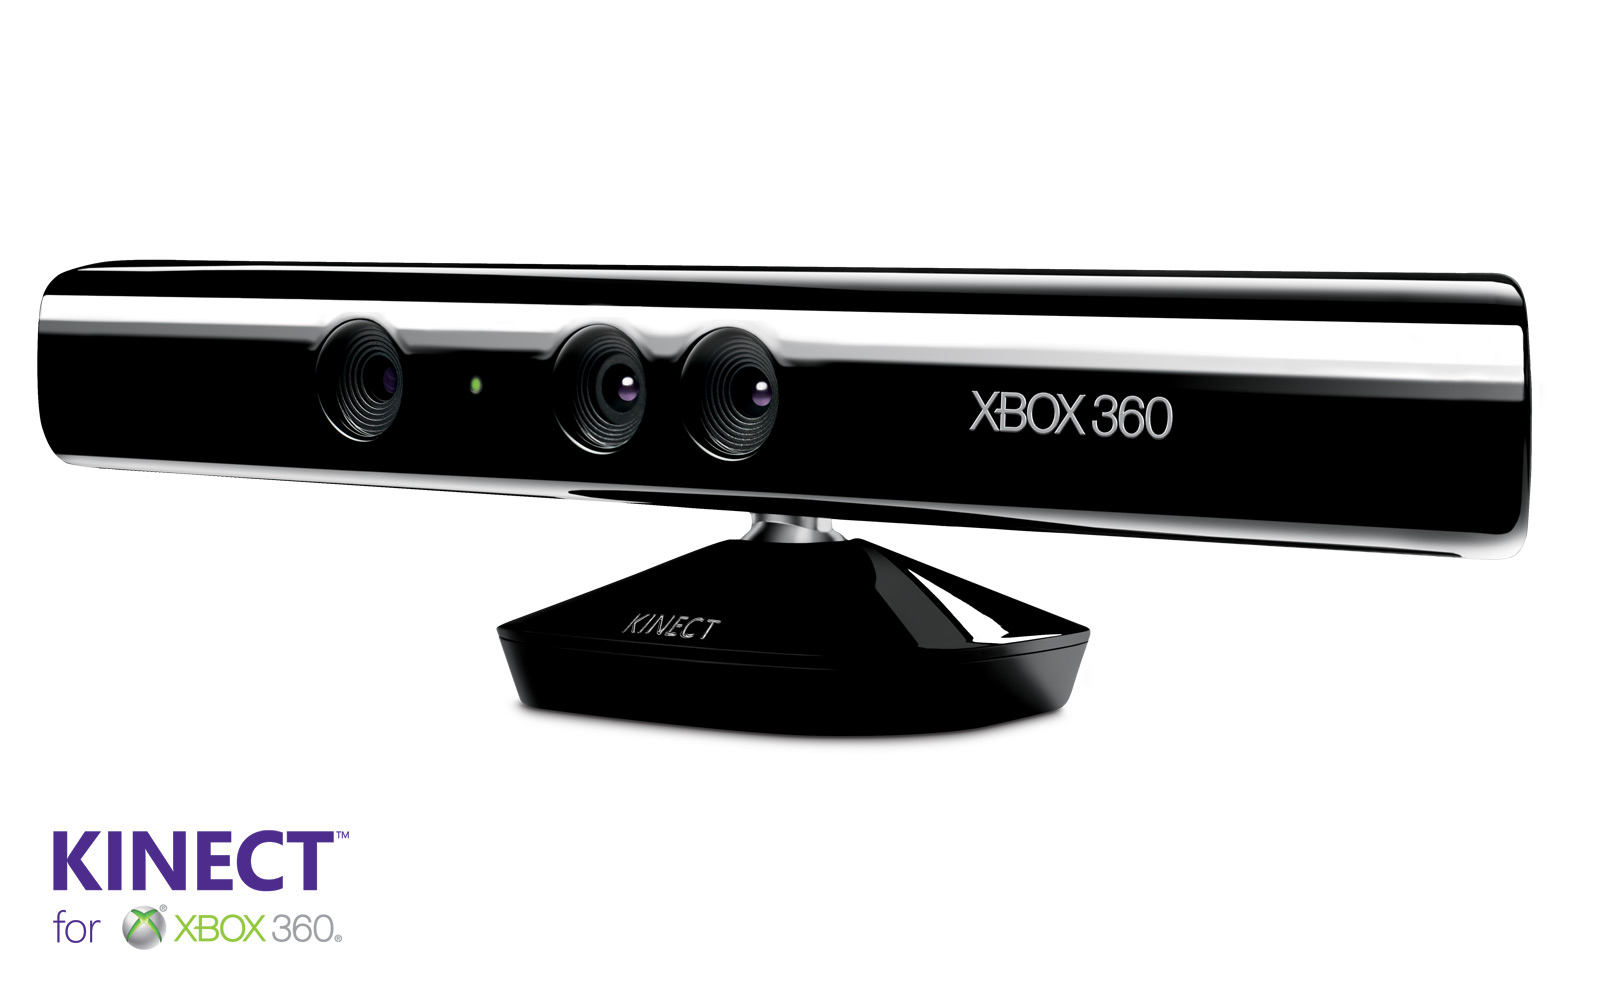
\includegraphics[width=70mm]{kinect.jpg}
\caption{The Xbox Kinect, the sensor on the left is the infrared light source, the center is a RGB camera and the 3D depth camera is on the right. in addition to these cameras, the base has a motorized tilt and a multi-array mic goes along the bottom of the wand.}
\label{kinectlable}
\end{figure}
\indent  The Kinect accomplishes this triangulation by using the known information about the sensor, the data obtained from the infrared projection and the image received from the camera. The sensor will project invisible light onto an object, the light bounces back and the infrared sensor reads back the data. These clusters of light that are read back can be matched to the hard-coded images the Kinect has of the normal projected pattern and allows for a search for correlations, or the matching points. While looking through the camera's focal point, the point of interest will fall on a specific pixel, depending on how close or far away it is, this means that we know along which trajectory this point is from the camera. The relative line of trajectory from the projector and from the camera, along with the known information about the distance between the cameras on the Kinect sensor, are used in the above described triangulation process to find the three-dimensional coordinates of the point. Figure ~\ref{kinectlable} shows how the three cameras are arranged on the Kinect.

% Bilateral Filter and Image Pyramiding
\indent In order to make this data more manageable, a bilateral filter is used to remove the erroneous measurements. This filter will just take every point, and recalculate the value of that point based on the waited average of the surrounding pixels in a specified neighborhood. The process takes away some of the sharpness of the depth map, but it removes the noise that will skew the results of the three dimensional reconstruction. The filter takes every pixel in the image and replaces its value with $BF[I]_{P} = \frac{1}{16} \left( \begin{array}{ccc}
1 & 2 & 1 \\
2 & 4 & 2 \\
1 & 2 & 1 \end{array}  \right) $ times the neighborhood of the 3 by 3 square of pixels around the pixel that is being changed. This resulting pixel value represents the average of the 9 pixels, where the closer pixels weight in the average is heavier than the further pixel values. Next, in order to represent the depth map in the true three dimensional points, a vertex must be created at each point where x, and y are the pixel values and the depth is the z coordinate. These points are then multiplied by a calibrated matrix to convert them into a vector map, or point cloud. The normal of each vertex is calculated by the cross product of the neighboring pixels. This process is combined with the process of computing a pyramid of the data, multiple copied of the depth map are made with smaller resolutions, at leach layer the vertices and their normals are calculated and stored. 

% Vector Field and Truncated Surface Distance Function
\indent The next step is to take a previously calculated vertex and normal map and run an Iterative Closest Point Algorithm on the four maps. This algorithm associates points by the nearest neighbor criteria, estimates a transformation using a mean square cost function, transform the point using the estimated parameter and then re-associates the points iteratively. This step creates a final rotation and translation that minimizes distant errors between the point clouds. This algorithm is useful because it will find the best way to position the point cloud before the reconstruction so that every part of the object is represented correctly. Once the best fit is found, the existing depth data can be combined with the existing model to get a more refined result. The filtering got rid of the noise, and adding the raw depth data back to this will add the important details back into the final model. A Truncated Surface Distance Function is used to fit the depth data and the model back together. Finally, a weighted average of the existing model and the latest depth measurements is taken and used to generate the surface using a ray-casting algorithm, to express the reconstructed object to the user. The model can be exported as an STL file to the Gcode converter, but some work still needs to be done in order to represent to the user what he ore she is trying to print. The ray-casting algorithm will tell a virtual camera looking at the virtual model what to display on the GUI. A ray is cast from every pixel in the image through the focal point of the digital camera, and the first surface that the ray intersects with is excited, displaying it to the user.  \cite{cite8}

%%%%%%%%%%%%%%%%%Image that shows raw depth data, filters and reconstructed object

% G-code Conversion
\indent { \bf G-code Conversion}\\ 
The RepRap firmware uses G-code to communicate to the 3D printer, specifically to define the print head movements. This code has commands that tell the print head to move to a certain point with rapid or controlled movement, turn on a cooling fan, or selecting a different tool. Since this 3D printer does not have as many features, the G-code generator does not have to add much complicated code, but rather just instructions to the printer head. Since the printer continuously dispenses plastic, it is necessary to find a path for it to take that will build up the reconstructed object layer by layer without placing too much plastic in any specific area. This requires cutting up the reconstructed object into layers and then finding the best path to traverse that layer without overlapping any part of that path. The G-code converter takes in the STL file, cuts it up into horizontal layers and then calculates the about of material that is needed to fill each slice. 



\section{Experimental Results}
%Measurements, repeated trials (for validation), error/performance analysis (as a function of system parameters). Include plots, images or tables to describe measurement values.

\begin{figure}[H]
\centering
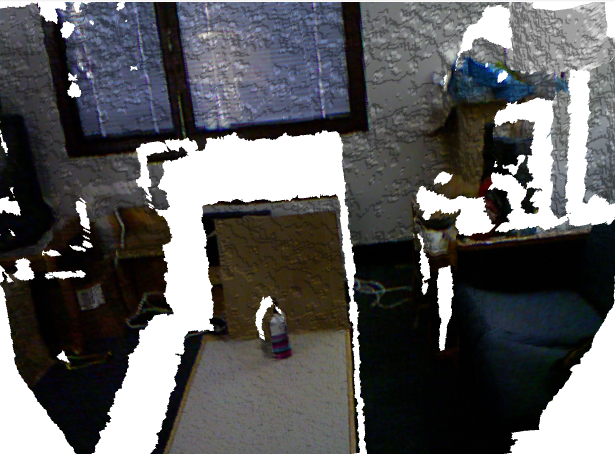
\includegraphics[width=70mm]{kinectwaterbottle.png}
\caption{The Kinect raw depth field, with the RGB image mapped to it, without bilateral filter}
\label{waterbot}
\end{figure}

\begin{figure}[H]
\centering
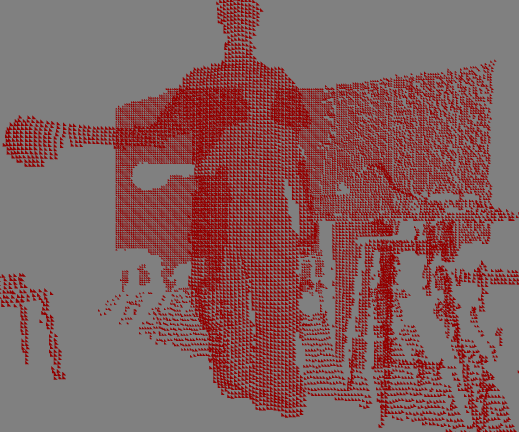
\includegraphics[width=70mm]{3dtriangles.png}
\caption{Triangles representing the 3D data}
\label{3dtri}
\end{figure}

\begin{figure}[H]
\centering
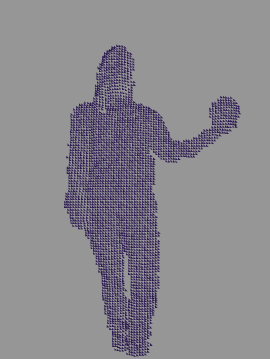
\includegraphics[width=70mm]{cadyholdingball.png}
\caption{The 3D data with the correct background filtered out}
\label{balls2}
\end{figure}

\begin{figure}[H]
\centering
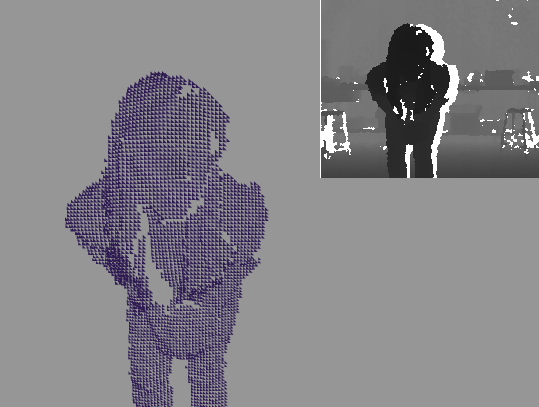
\includegraphics[width=70mm]{cadyholdingball2.png}
\caption{Comparison of the raw depth data and the Triangles that represent the 3D data}
\label{balls2}
\end{figure}




\section{Discussion}
%Discuss difficulties, sources of error, future work and extensions.
Part of the issue of working with this 3D printer was that many of the parts used in the construction of the machine were actually printed by another 3D printer. This meant that before we could start the construction of the printer, we had to wait on all of the correct parts to be printed. Even once we thought that we had all of the required pieces, we found two important parts that we were missing that we have to go to the Rutgers Maker Space to get printed. We also found that many of the plastic parts were made to be the exact size of the rods that needed to be placed into them, this meant that it took a lot of force to get some of the components to fit together properly. At one point we tried to use hot water to make the printed plastic more malleable but we fear that this made some of the pieces warp. \\
\indent Another big issues that was found with he construction of the 3D printer was the lack of good document ion on assembly. For the triangular base structure had to be taken apart and reassembles multiple time sin order to fix errors. One example was the motor bracket for the motor that controls the movement along the y-axis, there was not good diagrams to show which side of the machine this part should be placed and what direction it should be oriented. Figure~\ref{parts} shows a number of the unlabeled parts that we received from IEEE. Since documentation as hard to find and none of the parts were labeled, we also had trouble finding the correct STL files to send in in order to get ore parts. We knew that we were missing the brackets that connect the two top motors to the threaded rod that controls the movement along the z-axis, but we did not know what file needed to be printed.\\
\begin{figure}[H]
\centering
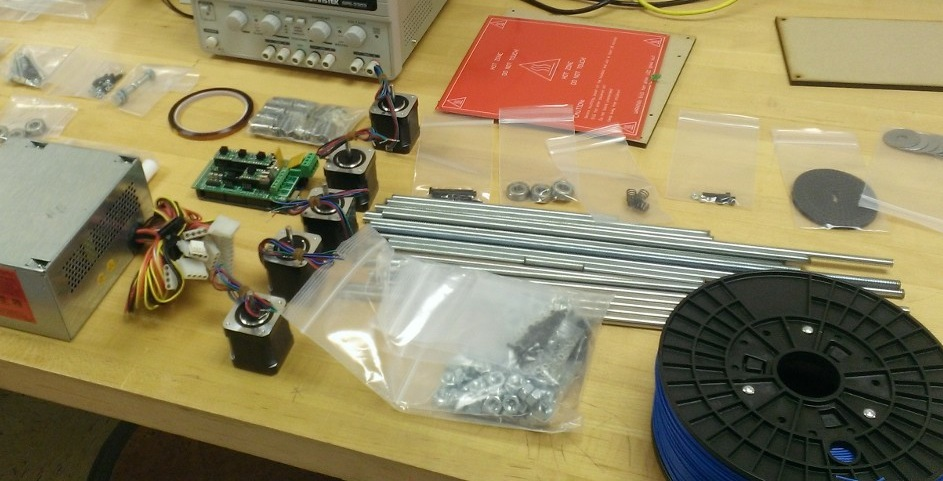
\includegraphics[width=70mm]{WP_20130223_002.jpg}
\caption{Parts of the 3D Printer}
\label{parts}
\end{figure}
\indent Even once the mechanical parts of the 3D printer have been constructed, we still need to calibrate all of the axes, add all of the electrical components, calibrate the firmware and build the protective frame around the printer. Figure~\ref{basebuilt} shows the constructed frame, x,y and z-axes and the installed printed. One of the issues that we will run into as we complete the 3D printer is the extruder. This component is responsible for heating and melting the ABS plastic and placing it onto the right place on the heat bed. We have discovered a problem that normal solder cannot handle the heat that is needed to melt the ASB plastic and the piece falls apart as the machine heats up. In order to fix this issue, we need to order silver solder that will be capable of withstanding a temperature of 221 degrees fahrenheit. 
\begin{figure}[H]
\centering
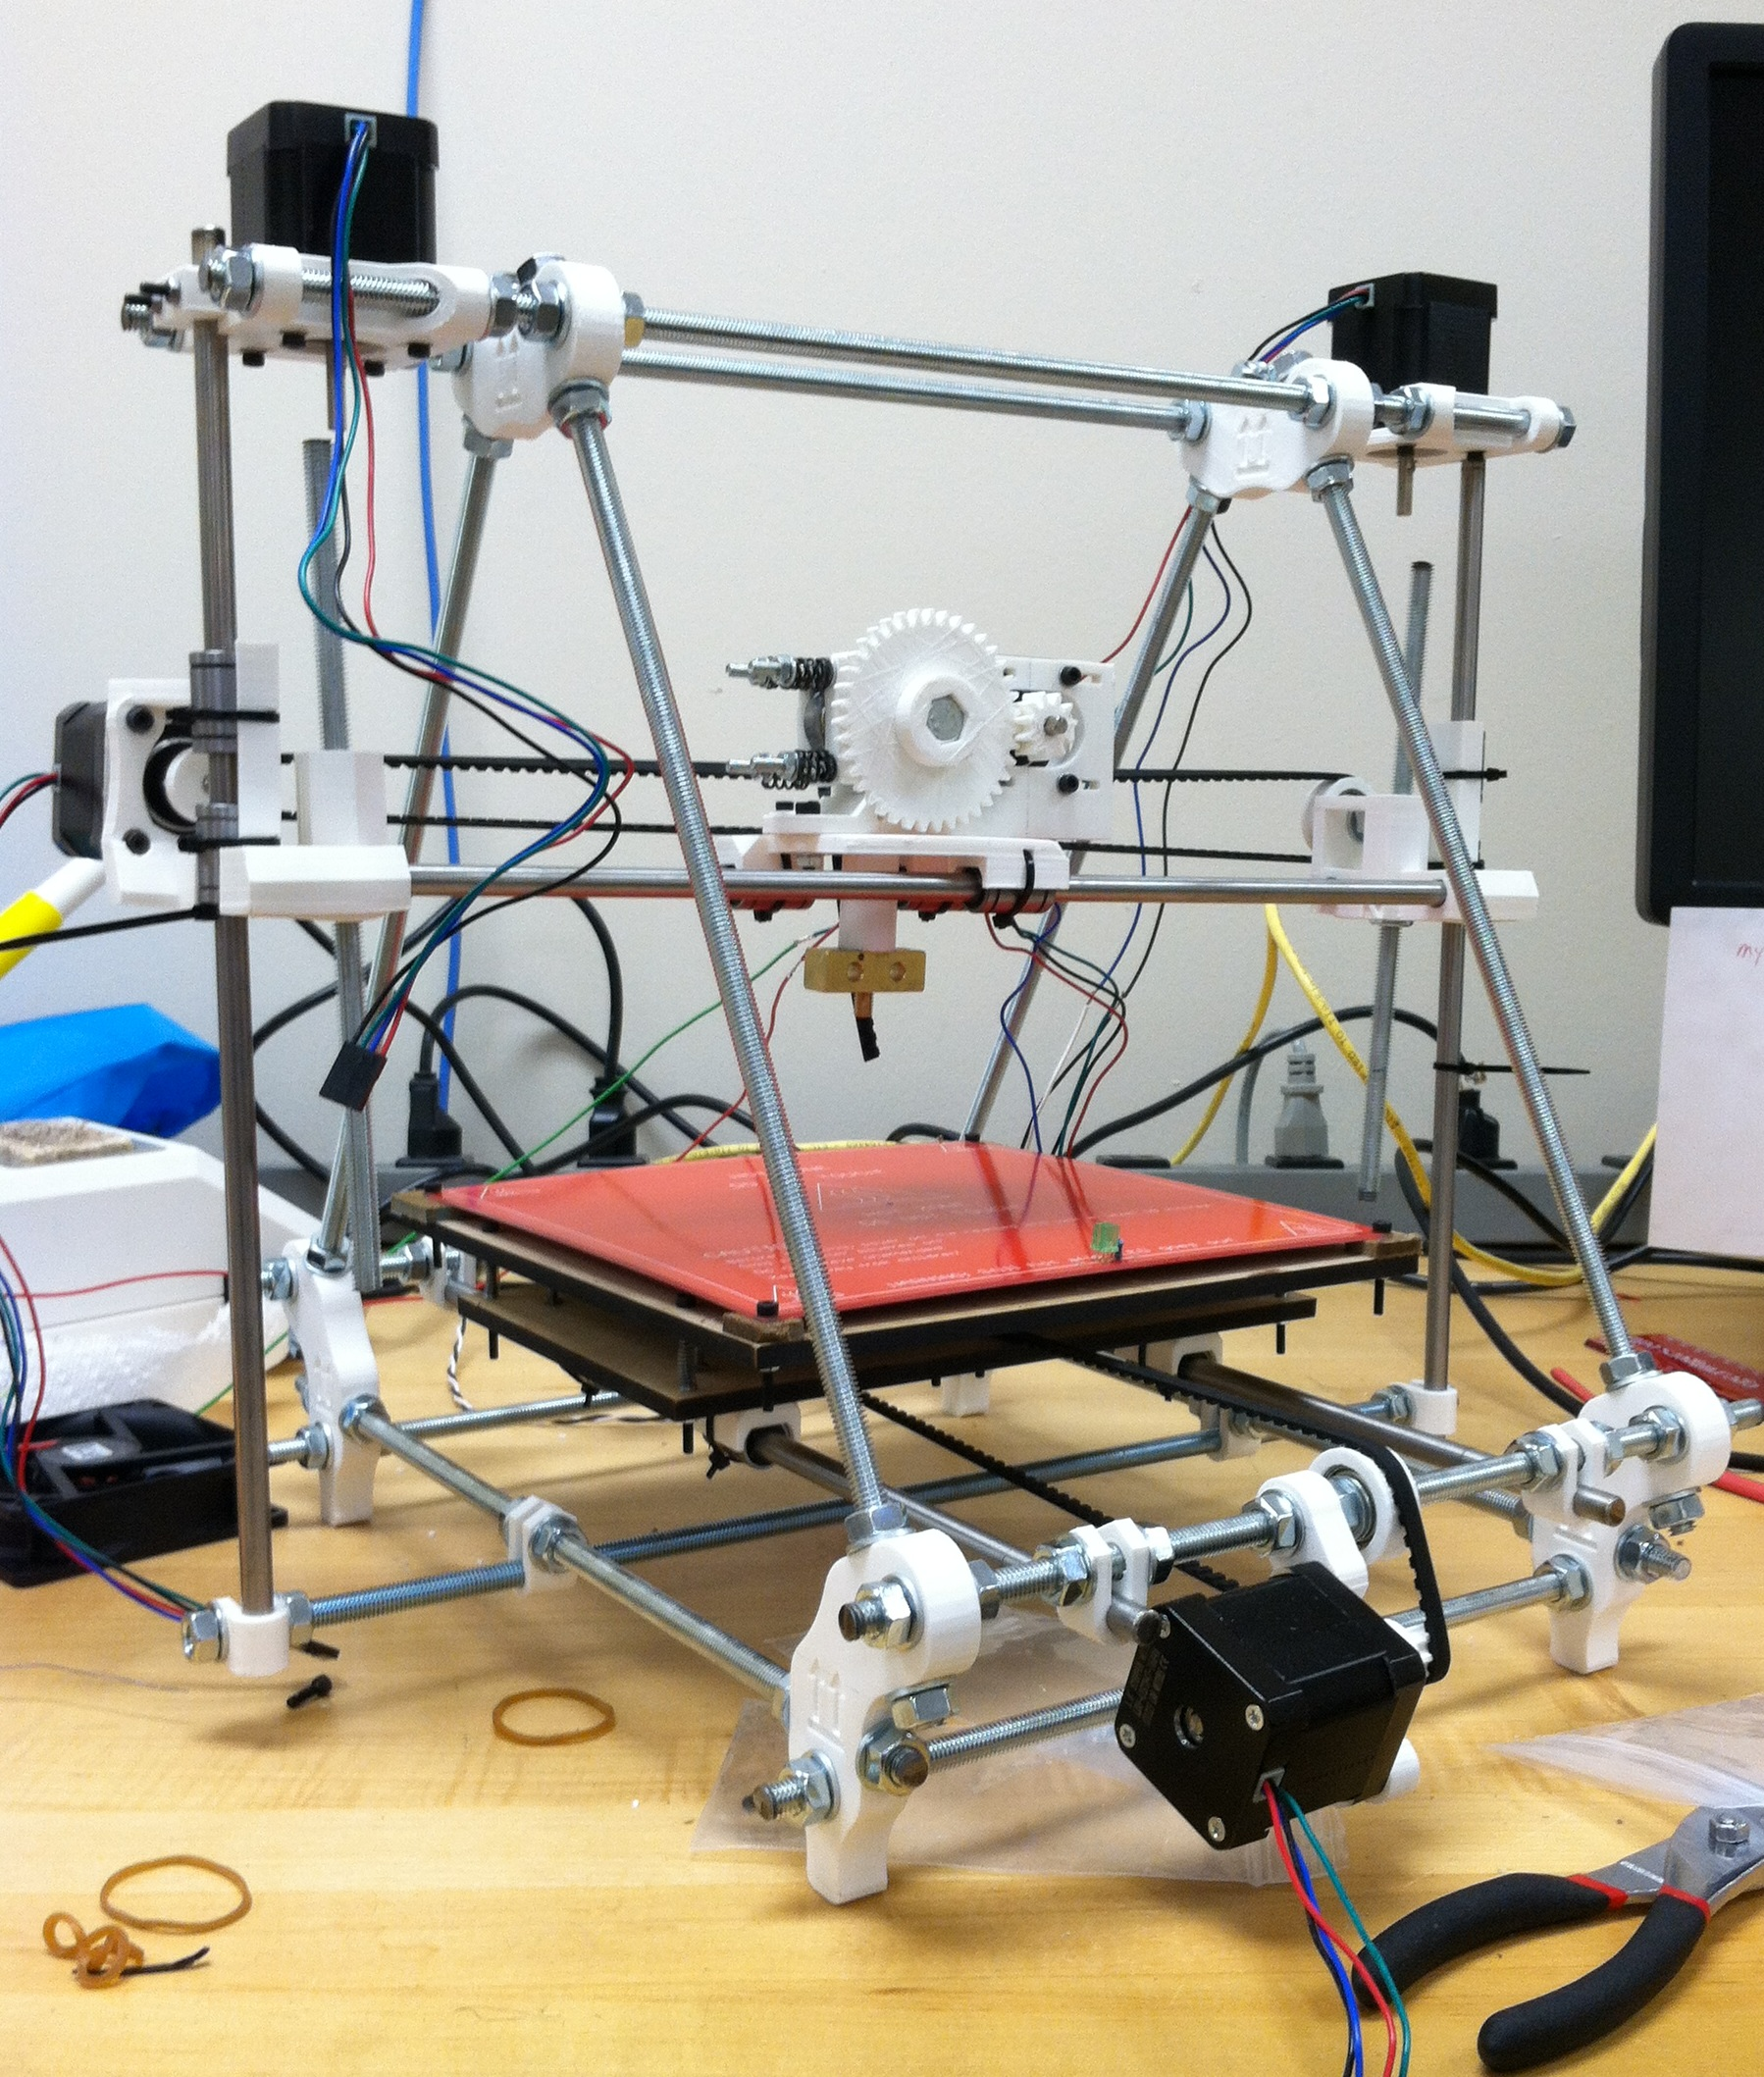
\includegraphics[width=70mm]{photo.JPG}
\caption{Construction of the 3D Printer Frame and x,y and z-axes}
\label{basebuilt}
\end{figure}

\indent 
The biggest issue that we have had with the software component of this project was the lack of examples. Other people who have worked on similar projects had been using the original version of the Microsoft Kinect Software Development Kit. This means that a many implementations used packages that are no longer part of the SDK that we have to work with. We've had to find ways to make the new SDK, which was released in 2012, work in a way similar to the old SDK. 

\section{Cost Analysis}
%Discuss the cost entailed with a product design based on your work. Use examples from currently available equipment in your cost estimates.
  \begin{description}
  \item[{\bfseries Printbot LC- \$ 549.00}] \hfill \\
  3D Printer for developing reconstructed objects
  \item{\bfseries [Microsoft Kinect- \$ 109.99}] \hfill \\
  The most powerful sensor for its price, contains color filtering and depth filtering in one package
  \item[{\bfseries 1kg 3mm ABS Spool-\$ 46.00}] \hfill \\
  Material that the 3D Printer uses for creating objects, spool is necessary for feeding into the printer
  \item[{\bfseries 2x 1lb 3mm ABS- \$ 36.00}] \hfill \\
  Extra printing material, no extra spool required
  \item[{\bfseries Arduino Leonardo-  \$ 24.95}] \hfill \\
  Microcontroller to plan orientation of object during reconstruction process
  \item[{\bfseries EasyDriver Stepper Motor Driver- \$ 14.95}] \hfill \\
  Allows the ability to control a stepper motion at lower voltages such as from an Arduino microcontroller
  \item[{\bfseries Stepper Motor with Cable- \$ 14.95}] \hfill \\
  Motor that can be controlled in "steps" this allows a more precise method for orienting objects being reconstructed
  \item[{\bfseries Total:}] \hfill \\
  {\bfseries \$ 795.84}
  \end{description}

\section{Current Trends in Robotics and Computer Vision}
% Describe real world robotic systems of research programs that are related to your capstone project. Research the literature and provide formal citations from publications (as obtained from IEEE Xplore or ACM Digital Library on the Rutgers library site) and periodicals (e.g. NY Times, Wall Street Journal). Do not use websites as sources for this section.

%Kinect Trends
One of the reasons that the Kinect has become so popular for computer vision projects is that it is a cheap, quick, and highly reliable for 3D measurements. Many researchers are beginning to look into the possibility of using this device to achieve everything from a 3D reconstruction of a scene to aiding in a SLAM algorithm. The fact that this device is so affordable, and so many new resources are available, makes the Kinect a viable device for conducting research in the field of robotics and computer vision.\\
%https://docs.google.com/file/d/0B6Kc0pBSSJ79UHF0U2h0d2E5NDQ/edit
\indent The KinectFusion Project is slightly different than other projects that were using the Kinect; instead of using both the RGB cameras and the sensor, this project tracks the 3D sensor pose and preforms a reconstruction in real time using exclusively the depth data. This paper points out that depth cameras aren't exactly new, but the Kinect is a low-cost, real-time, depth camera that is much more accessible. The accuracy of the Kinect is called into questions, the point cloud that the depth data creates does usually contain noise and sometimes has holes where no readings were obtained. This project also considered the Kinect's low X/Y resolution and depth accuracy and fixes the quality of the images using depth super resolution. KinectFusion also looks into using multiple Kinects to preform a 3D body scan; this raises more issues because the quality of the overlapping sections of the images is compromised. \\
%https://docs.google.com/file/d/0B6Kc0pBSSJ79eHdOZ2dxZ3JseW8/edit
\indent	Another KinectFusion Project is the Real-time 3D Reconstruction and Interaction, this project is impressive because the entire process is done using a moving depth camera. With this software, the user can hold a Kinect camera up to a scene, and a 3D construction would be made. Not only would the user be able to see the 3D Reconstruction, but they would be able to interact with it; for instance, if they were to throw a handful of spheres onto the scene, they would land on the top of appropriate surfaces, and fall under appropriate objects following the rules of physics. To accomplish this, the depth camera is used to track the 3D pose and the sensor is used to reconstruct the scene. Different views of the scene are taken and fussed together into a singe representation, the pipe line segments the objects in the scene and uses them to create a global surface based reconstruction. This project shows the real-time capabilities of then Kinect and why that makes it an innovative tool for computer vision.\\
%http://download.springer.com/static/pdf/111/chp%253A10.1007%252F978-1-4471-4640-7_1.pdf auth66=1362330926_cd812bb15c7056eaaf2e0d67d1235b82&ext=.pdf
\indent	 A study shown in the Asia Simulation Conference in 2011 demonstrated that a calibrated Kinect can be combined with Structure from Motion to find the 3D data of a scene and reconstruct the surface by Multi-view Stereo. This study proved that the Kinect was more accurate for this procedure than a SwissRanger SR-4000 3D-TOF camera and close to a medium resolution SLR Stereo rigs. The Kinect works by using a near-infrared laser pattern projector and an IR camera as a stereo pair to triangulate points in 3D space, then the RGB camera is used to reconstruct the correct texture to the 3D points. This RGB camera, which outputs medium quality images, can also be used for recognition. One issue this study found was that the resulting IR and Depth images were shifted. To figure out what the shift was, the Kinect recorded pictures of a circle from different distances. The shift was found to be around 4 pixels in the \emph{u} direction and three pixels in the \emph{v} direction. Even after the camera has been fully calibrated, there are a few remaining residual errors in the close range 3D measurements. An easy fix for this error was to we form a \emph{z}-correction image of \emph{z} values constructed as the pixel-wise mean of all residual images and then subtract that correction image from the \emph{z} coordinates of the 3D image.\cite{cite1} Though the SLR Stereo was the most accurate, the error e (or the Euclidean distance between the points returned by the sensors and points reconstructed in the process of calibration) of the SR-400 was much higher than the Kinect and the SLR. This study shows that the Kinect is possible cheaper and simpler alternative to previously used cameras and rigs in the computer vision field.\\
%http://download.springer.com/static/pdf/132/chp%253A10.1007%252F978-4-431-54216-2_24.pdf?auth66=1362331083_1772f4693c9be3cb7361c13d205fe417&ext=.pdf
\indent	Another subject of research that is looking into using the Kinect is the simultaneous localization and mapping algorithm, used to create a 3D map of the world so that the robot can avoid collision with obstacles or walls. The SLAM problem could be solved using GPS if the robot is outside, but inside one needs to use wheel or visual odometry. Visual odometry determines the position and the orientation of the robot using the associated camera images, algorithms like Scale Invariant Feature Transformation (SIFT), used to find the interest points, and laser sensors, used to collect depth data. Since the Kinect has both the RGB camera and a laser sensor, this piece of technology is a good piece of hardware to use for robots computing the SLAM Algorithm. In the study conducted by the students in the Graduates School of Science and Technology, at Meiji University, they found that the Kinect worked well for this process for horizontal and straight movement, but they had errors when they tried to recreate an earlier experiment, this means that their algorithm successfully solves the initial problem, but accuracy fell over time.\cite{cite2} They found that the issue was not with the Kinect, and that it could be solved using the Speed-Up Robust Feature algorithm (SURF) and Smirnov-Grubbs test to further improve the accuracy of their SLAM Algorithm. This study proved that the Kinect was a reasonable, inexpensive and non-special piece of equipment that is capable of preforming well in computer vision applications. \\
\indent	It seems as though the Kinect is a popular choice in current robotics and computer vision. This device is affordable, easily obtainable, and capable of a lot more than is expected from a video game add on. The Kinect combines a near-infrared laser pattern projector and an IR camera in one tool, and when combined with this eliminates the set up of some other configuration. The Kinect is also surprisingly accurate, requiring only some optimization software to make the results comparable to the results from a medium resolution SLR Stereo rig.\\
% 3D Printing Trends
%http://www.nytimes.com/2010/09/14/technology/14print.html?pagewanted=all&_r=0
\indent	One of the most innovated uses for the 3D Printer is its applications in the medical field. Since 2010, people have been using 3D printers to print out prosthetic limbs. One company in California has been printing the totally customizable prosthetics, which cost about one tenth of traditional prothetic limbs. Another company is looking at the possibility of using a 3D printer to print a house. Right now the design fits on the back of a tractor trailer and the 3D printer prints out custom concrete parts the are then assembled to complete the house. Some 3D printers have the ability to change the printing head, so it can begin printing with one material and then switch to a different material, all based on the code it receives, this means that a 3D printer could theoretically print the concrete part of the house and switch to printing the plastic siding or the glass windows all on the same path around the outside of the house. The most importunes aspect of these 3D printer applications is that it drastically cuts down on production costs, allowing the consumer to pay a lower price and get a completely customized product. Rather than paying a person to design the object, and then have a bother construct it, with a 3D printer all that needs to be done is the design and the 3D printer automates the entire construction process. For example, the 3D printed prosthetics cost 5,000 dollars to print and customize by covering the 3D printed material in a shoe or sleeve while a normal generic prothetic would cost about 60,000 dollars.\cite{cite5} The 3D printer is a piece of technology that could continue to make the price of consumer goods fall and allow for more customization than has ever existed for consumer products.
%http://www.popsci.com/science/article/2013-03/get-brand-new-skull-3-d-printing
 \indent In recent news, biomedical scientists have taken the 3D printing technology a step further than prosthetics. A man had 75\% of his skull replaced but a 3D printed implant made by Oxford Performance Materials. Plastics have been used since the 1940's to replace missing bone fragments, and 3D modeling techniques have been used to match the size and shape of the plastic to someones skull. This Connecticut based company combined the 3D modeling techniques with 3D printing technology to produce the replacement part that only took five days to fabricate.\cite{cite9} The material that it is printed with has some of the same properties as bones and are osteoconductive, so the skull will actually grow and attach itself to the implant. This is also much better than metals that would block doctors from seeing past the implant in X-rays. This company is now also looking at using this procedure to 3D print other replacement bones for victims or cancerous bone or trauma. \\
%http://p8080-140.234.1.9.proxy.libraries.rutgers.edu/EPSessionID=a1528ded19e99cdd2b1aebe7896ee2/EPHost=web.ebscohost.com/EPPath/ehost/detail?sid=e23287e9-aecd-4a83-bec6-90cedb7dace7%40sessionmgr4&vid=1&hid=22&bdata=JnNpdGU9ZWhvc3QtbGl2ZQ%3d%3d#db=ofm&AN=85463174
\indent Even though lower cost of production is a goal for many industries, the 3D printing technology can be considered a disruptive technology, meaning that over the course of a short period of time it could change an existing market and value network while replacing existing technology. An article in the Harvard Business Review explains that good would be produced at or close to their point of purchase or consumption. Even if this ins't the case with every industry, the cost will be offset by the elimination of shipping the completed object to the consumer, something like car parts could be printed in a metropolitan area rather than made and shipped from a factory. This article also mentions how the 3D printer would allow for cheap and efficient customization of these products. Since changing the shape, color or material of what you want to print is only a mater of changing code, the first model could be relatively different than the second model for virtually no extra cost. \cite{cite6} The 3D printer could potentially affect the global market. Many products are manufactured overseas since it is much cheaper for the pieces to be created an assembled by underpaid workers, when 3D printing is perfected the parts could be made and assembled by a machine in the US for less than it cost to have the product manufactured and shipped from overseas. 
%http://p8080-140.234.1.9.proxy.libraries.rutgers.edu/EPSessionID=e9758f18885b96365d7e86472d628a/EPHost=web.ebscohost.com/EPPath/ehost/detail?sid=2b6863d6-ae3a-4000-9104-efa71fbc900c%40sessionmgr14&vid=1&hid=24&bdata=JnNpdGU9ZWhvc3QtbGl2ZQ%3d%3d#db=ofm&AN=85517553
\indent	An article in Machine Design talks about what changes are being made to the 3D printers in order to make them more durable, user friendly and affordable. One brand, LeapFrog, has made the entire device out of aluminum and  replaced the stepper-motor drivers with professional drivers that last longer. This company has also added a duel option extruder so that the printer could construct something like a bridge by adding the plastic from one extruder and a water soluble support system with the other extrude that can be washed away once the printing is finished. This printer also uses PLA plastic, which is more brittle and has a lower melting temperature, can print smoother edges than the usual ABS plastic. Another brand, FormLabs, uses a liquid photopolymer instead of a spool of plastic, this resin cuts the price of printing materials in half and allows for a layer thickness of only 25 microns. The RepRap 3D printer has been designated a self-replicating printer because it can be used to print parts for constructing another 3D printer. It is believed that between 20,000 and 30,000 of these machines are now in existence.\cite{cite7} The company Staples has started "Staples Easy 3D" in Belgium and the Netherlands, where anyone can upload their file to the center and later pick up the 3D model at their local staples or have it shipped to their house. Services like this are a sign that 3D printing will soon be as mainstream as 2D printing. 


\section{}\bibliographystyle{plain}
\bibliography{FinalReport}

\section{Appendix} 
%Source Code: All source code (within reason) with some descriptive comments. The code does not count in the final page count
All of the source code for the Computer Vision-Based 3D Reconstruction for Object Replication Capstone Design Project can be found at: \url{https://github.com/KinectReplicator}

\end{document}
